\documentclass[12pt,a4paper,titlepage]{article}
\usepackage[latin1]{inputenc}
\usepackage{amsmath}
\usepackage{amsfonts}
\usepackage{amssymb}
\usepackage{braket}
\usepackage{graphicx}
\usepackage{subcaption}


\author{Tobias G\"oppel and Sophia Kronthaler}
\title{Theoretical Practical Course in Computational Physics}
\begin{document}

\maketitle

\newpage
\tableofcontents
\newpage

\section{Monte Carlo (MC) integration method} 

The Monte Carlo integration method is quite similar to the Riemann integration method with the subtle difference that one chooses the $x_i$s randomly. This leads to the following approximative formula for the integral:

\begin{equation}
I = \frac{b-a}{N} \sum_{i=0}^{N-1} f(x_i) \xrightarrow{N\rightarrow \infty} \int_a^b\! f(x)\, \mathrm{dx}
\end{equation}
												

We can estimate the integral of the function f by:

\begin{equation}
\int_a^b\! f(x),\mathrm{dx} \approx I \pm Error = V \braket{f} \pm V \sqrt{\frac{\braket{f^2}-\braket{f}^2}{N}} 
\end{equation}

Of course we do not know the standard deviation of f but we can approximate it "on the flight" when performing the Monte Carlo integration. In our program, we assume that the desired accuracy is
reached, when:
\[accuracy \geq \frac{\sqrt{\frac{\braket{f^2}-\braket{f}^2}{N}}}{\braket{f}} \]


As one can see, the error decreases with $\sim \frac{1}{\sqrt{N}}$.
To get an more detailed idea of what determines the error, we should notice that the individual function values at random points $x_i$ one the x-axis are themselvs random numbers.The Integrand, being sum of random numbers is a random number too. The distribution of the integrated values approaches a Gaussian. By using the central limit theorem it can be shown that the following expression holds:

\begin{equation}
\sigma^2(I_N) = \frac{V^2}{N} \int_V \!(f(x) - \braket{f})^2 \mathrm{dx}=\frac{V^2}{N}\sigma^2(f)
\end{equation}

This leads to the important conclusion that the variance of $I_N$ does not depend only on the quantity of random points $N$, but also on the volume $V$ and the variance of the function $\sigma^2(f)$.
To show this characteristic we define the ratio $\rho$.

\[\rho = \frac{N}{V^2}\frac{\sigma^2(I_N)}{\sigma^2(f)}\]
\newpage


\begin{figure}[h]
\centering
\caption{$f(x)=x$, volume: $[-1,1]$, ratio: 1.051}
	\begin{minipage}[b]{\linewidth}
		\centering
		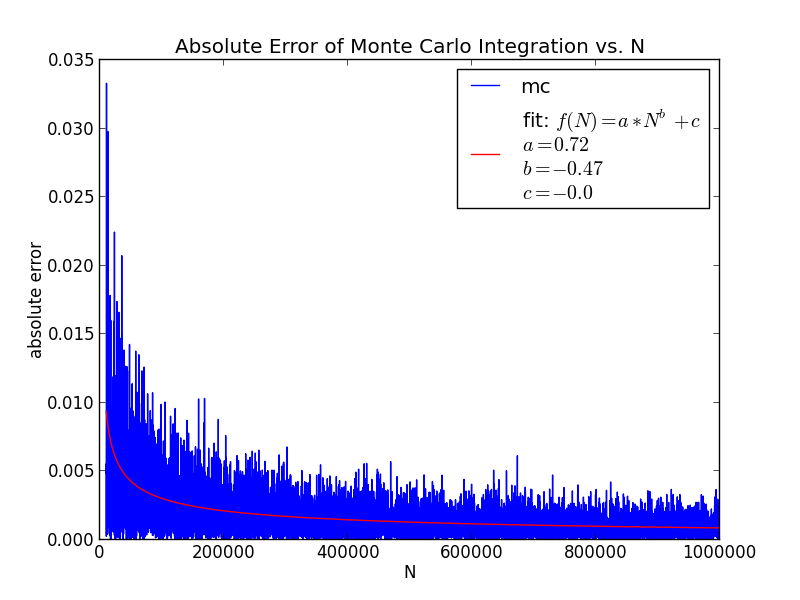
\includegraphics[width=\linewidth]{Plots/linear}
	\end{minipage}
	\begin{minipage}[b]{\linewidth}
		\centering
		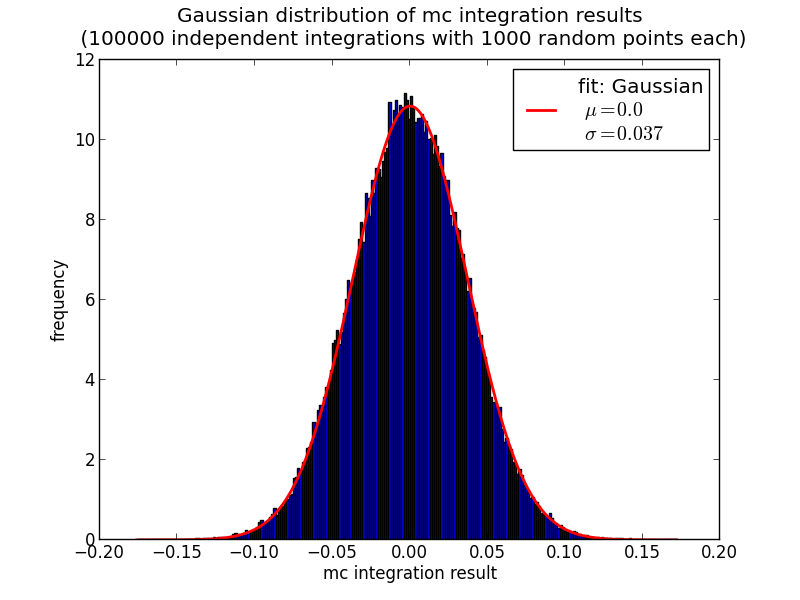
\includegraphics[width=\linewidth]{Plots/linearhist}
	\end{minipage}
\label{fig:linear}
\end{figure}
\begin{figure}[h]
	\centering
	\caption{$f(x)=x^2$, volume: $[-1,1]$, ratio: 1.043}
	\begin{minipage}[b]{\linewidth}
		\centering
		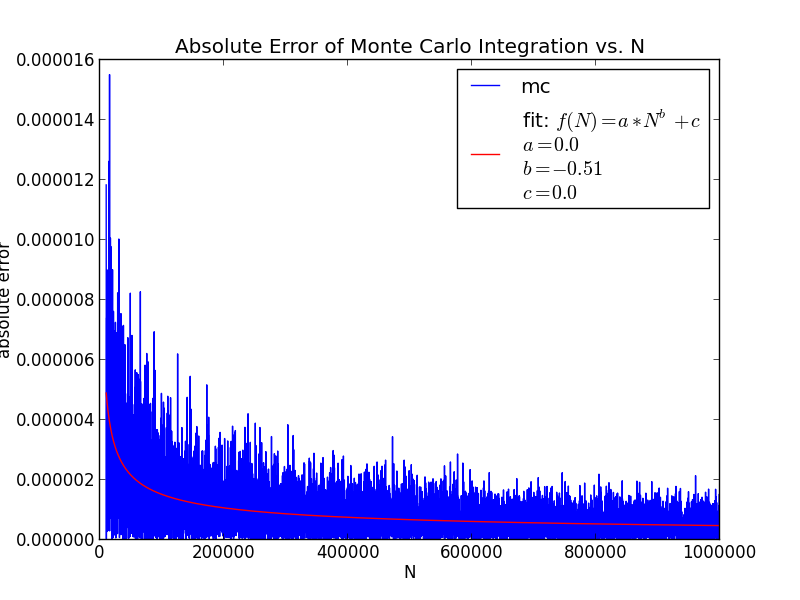
\includegraphics[width=\linewidth]{Plots/quadratisch}
	\end{minipage}
	\begin{minipage}[b]{\linewidth}
		\centering
		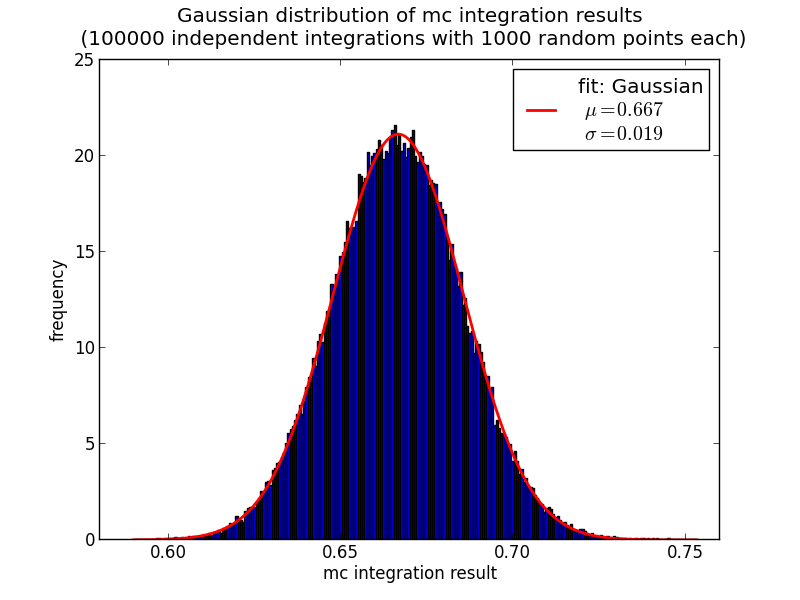
\includegraphics[width=\linewidth]{Plots/histQuadratisch}
	\end{minipage}
	\label{fig:linear}
\end{figure}
\begin{figure}[h]
	\centering
	\caption{$f(x)=x^5$, volume: $[-1,1]$, ratio: 0.951, (the fit function failed to find the correct fit paramters for the Gaussian)}
	\begin{minipage}[b]{\linewidth}
		\centering
		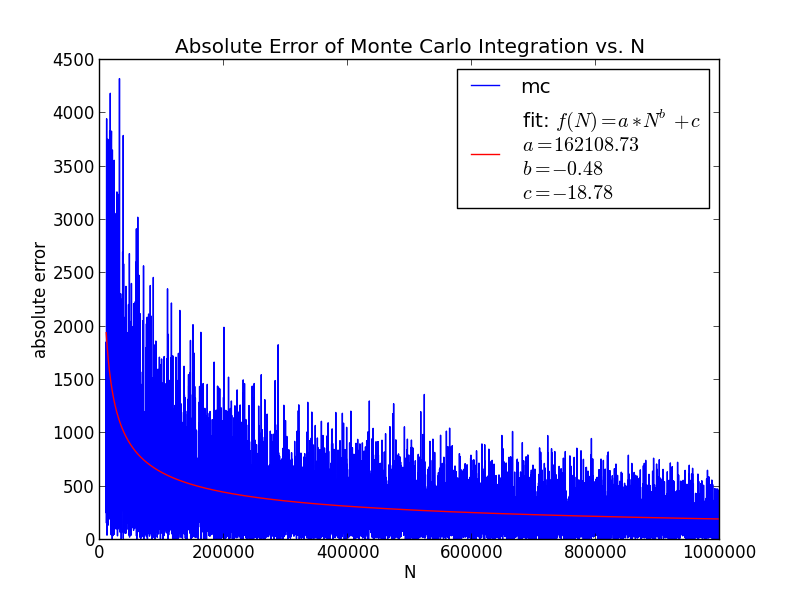
\includegraphics[width=\linewidth]{Plots/x5}
	\end{minipage}
	\begin{minipage}[b]{\linewidth}
		\centering
		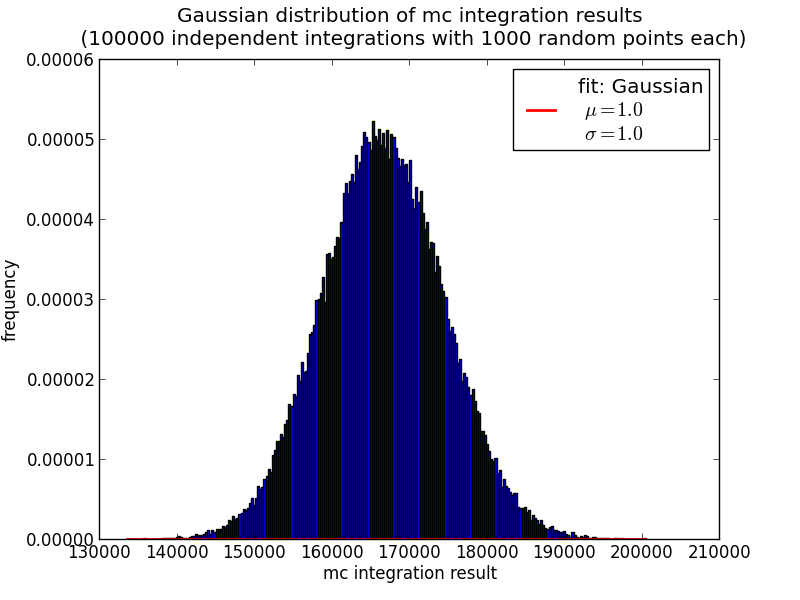
\includegraphics[width=\linewidth]{Plots/x5_HIST}
	\end{minipage}
	\label{fig:linear}
\end{figure}
\begin{figure}[h]
	\centering
	\caption{$f(x)=exp(x)$, volume: $[-1,1]$, ratio: 0.932}
	\begin{minipage}[b]{\linewidth}
		\centering
		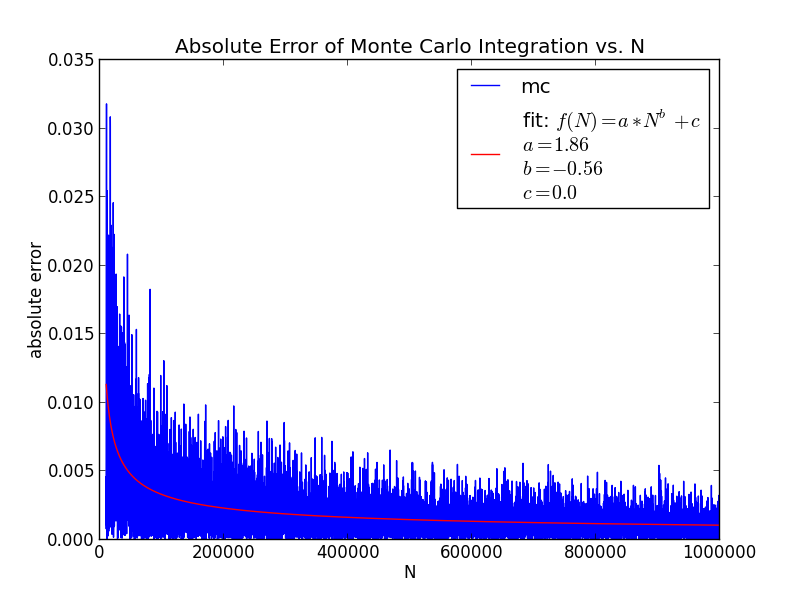
\includegraphics[width=\linewidth]{Plots/eFunktion}
	\end{minipage}
	\begin{minipage}[b]{\linewidth}
		\centering
		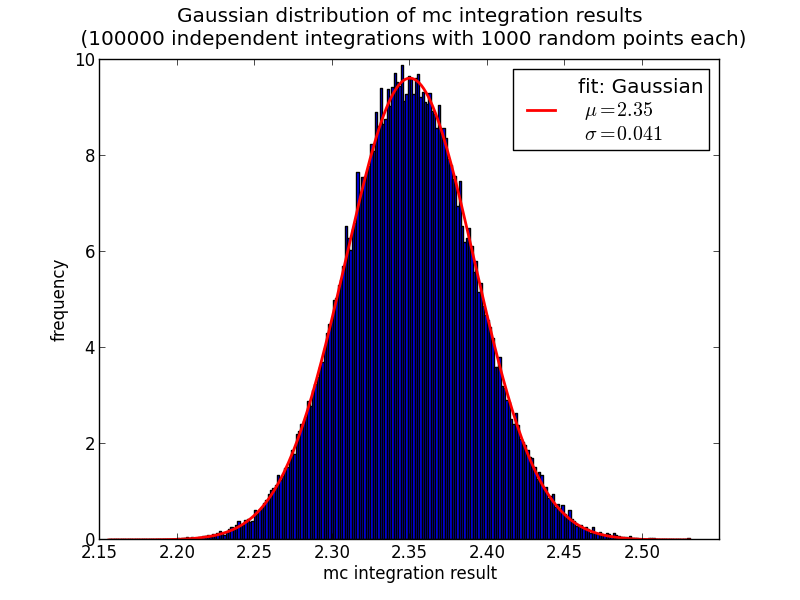
\includegraphics[width=\linewidth]{Plots/eFunktionHist}
	\end{minipage}
	\label{fig:linear}
\end{figure}
\begin{figure}[h]
	\centering
	\caption{$f(x)=sin(x)$, volume: $[0,2\pi]$, ratio: 1.085}
	\begin{minipage}[b]{\linewidth}
		\centering
		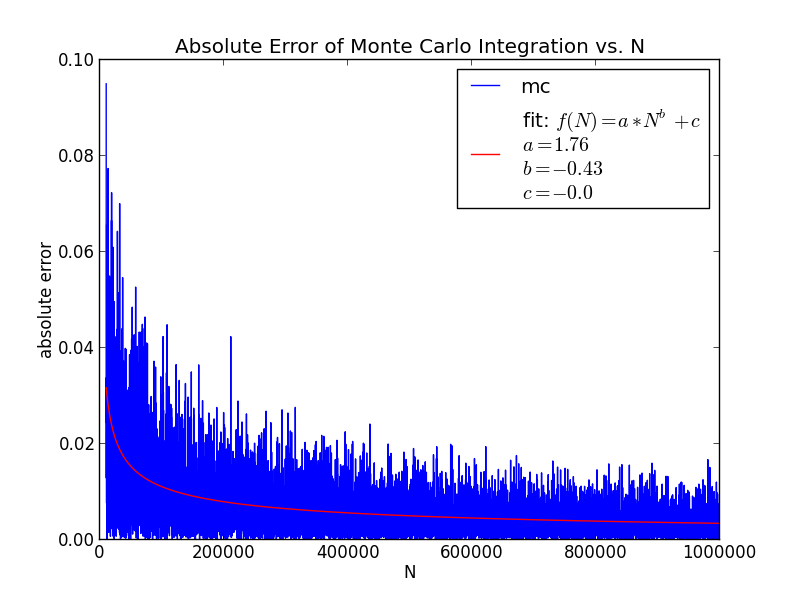
\includegraphics[width=\linewidth]{Plots/sin}
	\end{minipage}
	\begin{minipage}[b]{\linewidth}
		\centering
		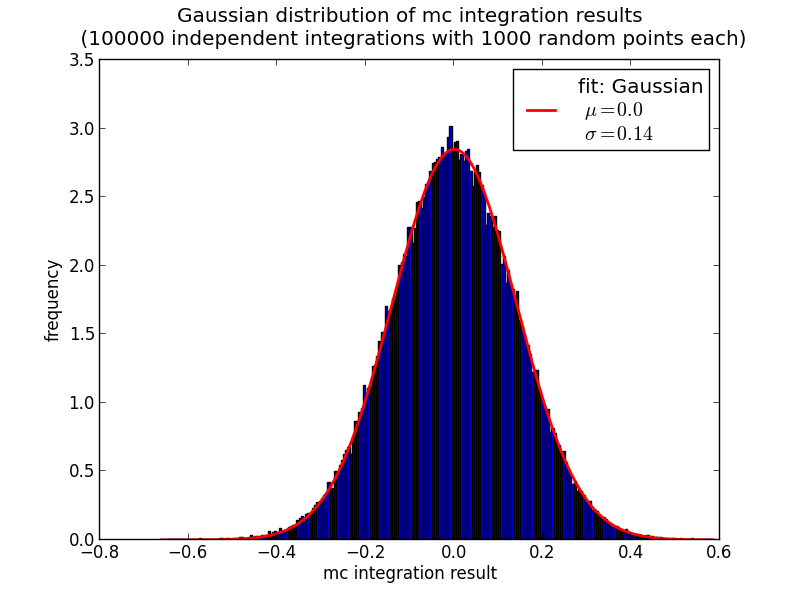
\includegraphics[width=\linewidth]{Plots/sin_hist}
	\end{minipage}
	\label{fig:linear}
\end{figure}




\end{document}